\documentclass{article}
\usepackage{graphicx} % Required for inserting images
\usepackage{enumitem}
\usepackage[margin=1in]{geometry}
\usepackage{algorithm}
\usepackage{algpseudocode}
\usepackage{amsmath}
\usepackage{csvsimple}
\usepackage{booktabs}

\title{BENG203 Assignment 2}
\author{Savan P Shah}
\date{April 2026}

\begin{document}

\maketitle

\textbf{Problem 1}

\begin{enumerate}[label=\alph*)]
    \item ecDNA cartoon
        \begin{figure}[h!]
        \centering
        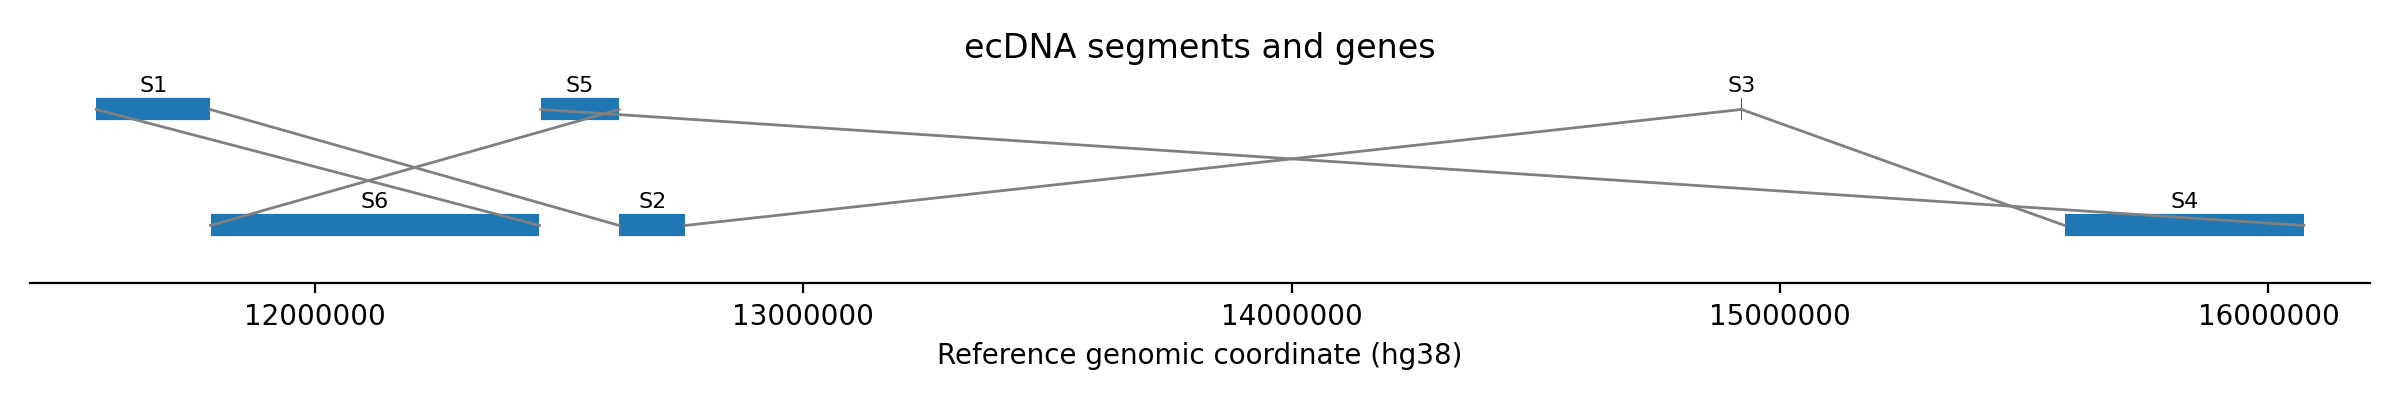
\includegraphics[width=1\textwidth]{ecDNA_cartoon.png}
        \caption{Segment S3 is small, and hard to resolve. The red coloring indicates that it is a (-) strand, so the end of segment S2 connects to the beginning of S3, and the beginning of S3 connects to S4.}
        \label{fig:cartoon}
        \end{figure}
    \item The gene with the highest expression is \textbf{DDX1} with an expression score of 8292.42 \\   
        DDX1 is the most expressed gene because its exonic regions have the highest cumulative expression signal in the ecDNA bedGraph data, producing a score far above the other candidate genes. This is biologically reasonable because DDX1 is a widely expressed RNA helicase that is frequently overexpressed in cancers, and amplified genes on ecDNA often show especially strong transcriptional output.\\
        This analysis uses the NCBI RefSeq - UCSC RefSeq (refGene) data, with a region defined by the provided ecDNA\_segments.bed file, and focuses on the provided genes. Expression scores for the other genes: \\
        LPIN1 expression score: 1457.57\\
        MYCN expression score: 3229.81\\
        TRIB2 expression score: 3106.50\\
        NTSR2 expression score: 0.23\\
        GREB1 expression score: 35.63\\
    \pagebreak
    \item Poisson Analysis Results ($\lambda=1578.80$)\\
        Number of significant higher-expression bins: 30\\
        Number of significant lower-expression bins: 81\\
        Total significant bins: 111\\
        \begin{center}
            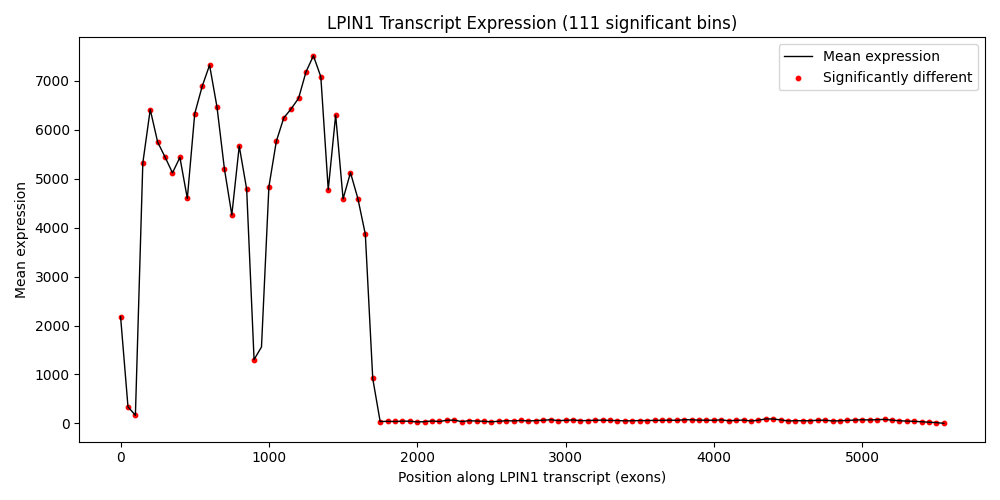
\includegraphics[width=.9\textwidth]{LPIN1_transcript_profile.png}
        \end{center}
    \item Yes, there was expression of several non-coding regions. Top 5 expressed non-coding regions:
    \begin{center}
    
          12716909-12723397, signal=616.500\\
          15586250-15634346, signal=605.738\\
          15908663-15947022, signal=286.098\\
          11773745-11827409, signal=131.441\\
          11771679-11773619, signal=85.078\\

    \end{center}
    These regions had significantly higher expression than two of the genes: NTSR2 and GREB1. Non-coding regions were defined using track ALL\_GENECODE49 and table wgEncodeGencodeCompV49, with a region defined by the provided ecDNA\_segments.bed file.

    \item 
    The structural rearrangement of ecDNA disrupts normal chromosomal organization in several ways that explain the dysregulation observed in parts (c) and (d). First, when two genomic segments are joined to form the ecDNA, TAD boundaries are broken and reassembled, allowing enhancers that were previously insulated from a gene to be placed in direct proximity. This can drive overexpression of genes like DDX1 and MYCN. Second, ecDNA can be present in tens to hundreds of copies per cell, all simultaneously transcriptionally active, multiplying expression far beyond normal levels. Finally, ecDNA lacks the higher-order chromatin compaction of normal chromosomes, making the entire structure constitutively accessible to transcription factors. This open chromatin state explains the non-genic expression observed in part (d): regions that would normally be silenced by compaction are now actively transcribed, producing enhancer RNAs or unannotated transcripts in intergenic and intronic space.
\end{enumerate}
\pagebreak
\textbf{Problem 2}\\
\textbf{BLAST} is a seed-and-extend local alignment tool designed for sensitive sequence similarity searching rather than ultra-fast read mapping. For fast filtering, it indexes short words from the query sequence, not the full database, and then scans the database for exact or high-scoring seed matches. The seed or word size is typically 11 for nucleotide BLAST and 3 for protein BLAST, with smaller words increasing sensitivity at the cost of speed. Once seeds are found, BLAST extends them into high-scoring segment pairs, and later improvements such as two-hit triggering and gapped BLAST reduced unnecessary extensions while allowing insertion/deletion-aware alignment. Because of this design, BLAST is aimed at retrieving not only highly similar sequences but also more moderately or distantly related homologs, especially in protein searches where evolutionary similarity may persist despite substantial divergence.\\
\textbf{BLAT} is a fast seed-and-extend alignment tool designed mainly for finding highly similar sequences, especially within the same species or among closely related species, rather than for detecting distant homology. For speed, BLAT indexes the database rather than the query, typically keeping a hash table of non-overlapping genome k-mers in memory, so queries can be scanned rapidly against a prebuilt genome index. In nucleotide mode, BLAT commonly uses 11-mers, while protein searches use short amino-acid words such as 4-mers; more generally, its k-mer sizes are chosen to favor exact or near-exact matching rather than highly permissive seeding. Algorithmically, BLAT improves speed by clustering multiple nearby seed hits before performing detailed alignment, and it can stitch aligned blocks together across exons, which makes it especially useful for cDNA, EST, and transcript-to-genome mapping. Because of this design, BLAT is aimed at retrieving matches with very high identity, such as roughly 98\% for same-species cDNA-to-genome alignments and substantially lower but still strong similarity for related-species protein comparisons, rather than the more remote homologs that BLAST is meant to find.\\
\textbf{Bowtie2} is a fast read aligner designed primarily for mapping short, relatively accurate sequencing reads to a known reference genome, making it well suited for Illumina-style data rather than distant homology searches. For rapid filtering, it indexes the database/reference genome using an FM-index derived from the Burrows–Wheeler transform, which allows memory-efficient substring searches instead of scanning the genome directly. It uses a multiseed strategy with seeds of roughly 20–22 bases by default, placing several seeds along each read so candidate mapping locations can be found even when the read contains a few mismatches or small indels. After seeding, Bowtie2 applies efficient dynamic programming for gapped alignment and improves on the original Bowtie by supporting local as well as end-to-end alignment, affine gap penalties, and better handling of insertions and deletions. Because of this design, Bowtie2 is aimed at retrieving high-similarity matches between sequencing reads and a reference genome, typically when reads are expected to differ only modestly from the target due to sequencing error, small variants, or limited divergence.\\
\textbf{Minimap2} is a versatile sequence aligner designed mainly for long, error-prone reads and long genomic or transcript sequences, so it is especially well suited for Oxford Nanopore and PacBio data rather than classic short-read mapping. For fast filtering, it indexes the database/reference using minimizers, which are representative k-mers selected from sliding windows, instead of storing every possible k-mer; this makes the index compact and efficient for long-sequence search. The query is therefore not the primary indexed object: minimap2 takes minimizers from each query sequence as seeds and matches them against the prebuilt reference index, with typical presets using k-mer lengths around 15 to 19 depending on the application. Algorithmically, minimap2 improves on older seed-and-extend mappers by using a seed-chain-align strategy, where exact seed matches are first chained into colinear anchor sets and only then refined with base-level dynamic programming, while additional heuristics such as concave gap costs, split-read alignment, and Z-drop help it handle long indels, structural variation, and spliced mappings efficiently. Because of this design, minimap2 is aimed at retrieving high-similarity matches between long queries and a reference even when the reads contain substantial sequencing error, and it has become a standard tool for long-read mapping, transcript alignment, and overlap detection in assembly workflows.

The alignment target determines what kinds of matches the algorithm must recover, and that choice drives both parameter settings and overall algorithm design: if the goal is to find homologs in a related species, the method must tolerate evolutionary divergence, so it typically uses shorter or more permissive seeds, substitution-aware scoring matrices, lower thresholds for extending hits, and local alignment strategies that can recover conserved regions even when the full sequences are not highly similar. By contrast, if the goal is to map human RNA to the human genome, the expected sequence identity is usually high, so the algorithm can use longer seeds, stricter mismatch filters, and more aggressive pruning for speed, but it must also be designed to handle exon–intron structure, which means splice-aware chaining and gap models that recognize long introns rather than treating every gap as a simple indel. More generally, as the expected similarity decreases, aligners must spend more computation on sensitivity because many true matches would be missed by strict seeding, whereas when the expected similarity is high, the algorithm can prioritize speed and precise placement because the correct mapping is easier to distinguish from noise.\\
\newpage
\textbf{Problem 3}\\
\begin{enumerate}[label=\alph*)]
    \item Since the bloom filter has $m$ bits, the probability of one specific bit being set is $\frac{1}{m}$ and the probability of that bit not being set is $1-\frac{1}{m}$. Considering $n$ objects, each setting $h$ bits, there are $hn$ placements total. This means the probability of a chosen bit being missed after all placements is:
    $$(1-\frac{1}{m})^{hn}$$
    Complementary to that, we can see that the probability of a chosen bit being hit at least one time is given by:
    $$1-(1-\frac{1}{m})^{hn}$$
    A false positive for object o would require h bits to be set, yielding the probability:
    $$P_{FP} = (1-(1-\frac{1}{m})^{hn})^h$$
    \item 
    Minimizing the above probability proves difficult, so an approximation is used. With a sufficiently large bit string length $m$:
    $$(1-\frac{1}{m})^m \approx e^{-1}$$
    Using this approximation, we can simplify the probability to:
    $$P_{FP} = (1-e^{-\frac{hn}{m}})^h$$
    We can then minimize $h$:
    $$\ln(P_{FP}) = h\ln(1-e^{-\frac{hn}{m}})$$
    Differentiate with respect to $h$, set $f'(h)=0$ to minimize $P_{FP}$, and solve:
    $$\ln(1-e^{-\frac{hn}{m}}) + h\frac{d}{dh}[\ln(1-e^{-\frac{hn}{m}})] = 0$$
    $$h = \frac{m}{n}\ln 2$$
    \item 
    To derive the lower bound for m, we substitute our optimized $h$ into our approximated $P_{FP}$.
    $$\ln(P_{FP}) = h\ln(1-e^{-\frac{hn}{m}})$$
    $$\ln(P_{FP}) = \frac{m}{n}\ln 2\ln(1-e^{-\frac{\frac{m}{n}n\ln 2}{m}})$$
    Our exponent reduces:
    $$e^{-\frac{\frac{m}{n}n\ln 2}{m}}=-e^{-\ln2}=-\frac{1}{2}$$
    Giving us the expression:
    $$\ln(P_{FP}) = \frac{m}{n}\ln 2 \ln(\frac{1}{2})$$
    Therefore, $$m \geq -\frac{n\ln(P_{FP})}{(\ln2)^2}$$
    \begin{center}
        \csvreader[
        tabular=cc,
        table head=\toprule P\_FP & min\_BF\_size\_kB \\ \midrule,
        late after line=\\,
        table foot=\bottomrule
        ]{BF_size_error.csv}{}%
        {\csvcoli & \csvcolii}
    \end{center}

    \item 
    
    
\end{enumerate}


\end{document}
